\documentclass[12pt]{article}

\usepackage{setspace}
\usepackage{hyperref}
\usepackage{graphicx}
\usepackage{url}
\usepackage{xcolor}
\newcommand\todo[1]{\textcolor{red}{#1}}

\onehalfspacing

\parskip=2ex
\parindent=2em

\title{SWEN439 Visualisation Essay \\ John Snow's Cholera Map}
\author{Hai Tran 300224467}
\date{\today}

\begin{document}
\maketitle 

%Optional abstract
\begin{abstract}

\end{abstract}
\textcolor{red}{
You will pick a visualisation and write an essay about that visualisation. 
You can do the cholera map, then show other things that were similar at the time, and for future show what visualisations came after that resemble it. Like dot maps. They would be not the main topic, but just an example of modern visualisations that are similar or you can contrast it with modern visualisations for disease spread to show how we do the same thing these days but use perhaps different visualisations.
}

\begin{itemize}
\item A clear description of the visualisation and how to read / interpret it
\item What questions does this visualisation address effectively and which does it not?
\item Is this a visualisation that is easy to use for novice viewers, or is it more intended for experts?
\item What is the history of the visualisation? Where did it come from? Where is / was it used?
\item What is the current state of research with respect to this visualisation?
\end{itemize}

\section{Introduction}
% This essay introduces John Snow's Cholera map, the history behind it, and the current state of research with respect to Snow's visualisation. 

This essay explores an influential visualisation created by John Snow in the nineteenth century known as the Cholera Map. During this time, many outbreaks of cholera occurred - a deadly infectious disease was thought to be spread via miasma, causing many deaths. This essay explores the history of John Snow's cholera map, how it came to be, the influence and contributions it had on the visualisation field, the questions it addresses, and the current state of research with respect to Snow's map. 

\section{The History of John Snow's Cholera Map}

In the nineteenth century, thousands of lives had been lost due to a disease called cholera. Although unknown at the time, cholera is caused by a bacteria called Vibrio cholerae, doubling in number every thirteen minutes and attacking the stomach and intestines \cite{channel1}. Symptoms include severe vomiting and diarrhea in victims, eventually causing an agonizing death to the victim in a matter of hours \cite{heros, channel1}. During the time of the nineteenth century, there was no cure for cholera and no one knew what caused the disease. Doctors were convinced cholera was contracted through miasma: harmful airborne odours emanating from decaying waste, repulsive sewage or ``foul-smelling sites of organic decay" \cite{ucla, test}. This theory was based on observations that showed poorer areas being more susceptible to cholera, deaths in these regions more frequent \cite{heros}. However, a physician by the name of John Snow had an opposing view. Snow disbelieved the idea of cholera being caused by miasma, instead, hypothesising that cholera was a waterborne disease. In particular, Snow believed that cholera was caused by water that was contaminated by sewage \cite{ucla}. Snow came to this hypothesis after previously studying various outbreaks of cholera, writing academic papers that discussed his findings, yet no one believed him \cite{original}. Scientists and doctors gave little attention to Snow's work and were not convinced in Snow's theory, despite his findings \cite{ucla}. 

During the nineteenth century, 2.5 million people were estimated to be living in London. It was the largest city that had been built and contained the largest population at the time \cite{channel1, tedtalk}. An estimated third of the population lived in slums, up to 8 people in a room, and up to 40 to a house. Due to such a large population, this provoked filthy and unsanitary living conditions. People had cesspools containing fecal matter in their basements, eventually accumulating overtime. All this supported the idea that cholera was caused by miasma in the atmosphere caused by unsanitary living conditions. In an attempt to mitigate the smell, authorities created a law that made citizens empty their cesspools, expecting this to prevent cases of cholera \cite{tedtalk, johnson}. 

On the 28th of August, 1854, a cholera epidemic had broken out in the Soho district of London, England \cite{tedtalk}. After 3 days, 127 were found dead in London due to the epidemic. Within a few weeks, around 600 were estimated dead \cite{youtube, tedtalk}. Snow described it as ``the most terrible outbreak of cholera which ever occurred in this kingdom" \cite{ucla}. Snow lived in the Soho district near the cholera outbreak and wanted to investigate his hypothesis of cholera being a waterborne disease. He suspected that if his hypothesis were true, incidents of the disease would involve a single source that everyone was going to, incidents of cholera clustering around the source of contamination such as a specific water pump \cite{test, tedtalk, johnson}. 

Snow tested his hypothesis by interviewing locals about cases relating to cholera with the help of Reverend Henry Whitehead. With the help of Whitehead, a socially connected individual, Snow was able to track down most cases of cholera \cite{tedtalk}. Snow searched for patterns, analysing data collected from the interviews, asking locals whether they knew if the victims had drunk from a specific water source, or whether they had not. He increasingly found people who drank from the Broad Street water pump were getting sick, and people who did not, were not getting sick. He also found that a brewery located near this pump had an independent water source where workers were not contracting the disease \cite{blog}. With further investigation, Snow found that the brewery workers were drinking beer rather than water which further supported his hypothesis \cite{youtube}.

Snow thought of representing this data as statistics in a table, but eventually had the thought to do a visualisation which provided a high level view of the statistical information that he wanted to display \cite{tedtalk}. Snow plotted data on a map containing water pumps, and every death from cholera that he had collected to see if there was a pattern. He found that 578 deaths had occurred near the Broad Street water pump in a small neighbourhood \cite{channel1}. Snow also noticed outliers from the information he collected such as a victim by the name of Susanna Eley that had contracted cholera but lived far away from the Broad Street pump. With further investigation, Snow found out that Eley had moved from Broad street and preferred the water from the Broad Street pump. For these reasons, her son sent her a daily supply from the pump \cite{channel1}. 

Statistical analysis of the data collected and the visualisation led Snow to track the origin of the outbreak in the Soho district to the Broad Street water pump \cite{test}.
Snow provided his research to authorities, which were still sceptical about his findings. Despite this, On the 8th of September 1854, authorities decided to remove the handle from the Broad Street pump as a trial due to Snow's research \cite{ucla, youtube}. Coincidentally, the cholera outbreak stops. Although Snow had the pump handle removed, the cholera epidemic had already been on the decline. It is not certain that removing the handle stopped the outbreak, as opposed to the outbreak naturally burning itself out \cite{original}.

Although Snow was able to trace the cases of cholera back to the Broad Street pump, Snow could not prove what caused the contamination of the water in the first place \cite{ucla}. It was later discovered the water pump was located only three ft away from an old cesspit which leaked sewage into the water supply \cite{channel1, heros}. The old cesspit contained fecal matter from a babies diaper that had been dumped into it. The baby had contracted cholera from an unknown source, and had caused the 1854 outbreak \cite{heros, tedtalk, johnson}. 

By 1866, when the next cholera outbreak had broken out, authorities had been successfully convinced by John Snow's map, and warned everyone to start boiling their water. This was ``the last time that London had seen a cholera outbreak since" \cite{tedtalk}. John Snow's method of mapping statistic data to visualise the spread of the disease is still used today \cite{channel1}. 

\section{John Snow's Cholera Map}

John Snow's map was based on the recorded cholera deaths that Snow had investigated in the Soho district of London, and was hand drawn by Snow himself. The map was a bird's eye view of neighbourhoods in the district containing information about cases that he had collected from the cholera outbreak. Since Snow was particularly interested in whether cholera was a waterborne disease, he decided to map water pumps that were of interest to him, drawing black circles representing the locations of each water pump on the map. For each water pump, he labelled ``PUMP" in capitalised text. This not only allowed him to test his hypothesis, it enabled Snow to visualise the information in a meaningful way. If his hypothesis were true, then it was expected deaths from the cholera outbreak would cluster around a particular source. Snow made his map large enough to encapsulate water pumps in other vicinities, to see if there was a relationship between cholera being a waterborne disease. By doing this, it enabled Snow to distinguish and investigate any outliers, or abnormalities in the outbreak which could be visualised on Snow's map \cite{blog}. Snow plotted each case of cholera on the map, drawing thin black strokes which formed horizontal bars. Each bar represented a death in the neighbourhood caused by cholera \cite{tedtalk}. Stacked horizontal bars similar to the bars of a bar chart, represented multiple deaths at a particular address ``like a pile of little corpses" \cite{blog}.

\todo{Fix this} Since no one had listened to Snow, Snow created the map to convince the general public that , particularly authorities. John Snow's map is relatively easy to understand. All the domain knowledge needed, was to understand what the symbols represented, which were the black circles and horizontal bars.

Through the visualisation of the map, the message was evident. There was a significant amount of deaths clustered around a water pump on Broad Street. Deaths further away from the map seemed to be less frequent, clearly demonstrating ``something poisonous emanating out of this pump on the map" \cite{blog}.

John Snow was able to convince authorities that the cause of the outbreak may have been the Broad street water pump. Authorities later removed the handle from the water pump, and later, in 1896, when another outbreak had occurred, authorities instructed locals to boil their water. 

The significance of Snow's map had changed the way we visualise disease such that ``many have said changed medicine forever". \cite{heros}

\begin{figure}
\centering
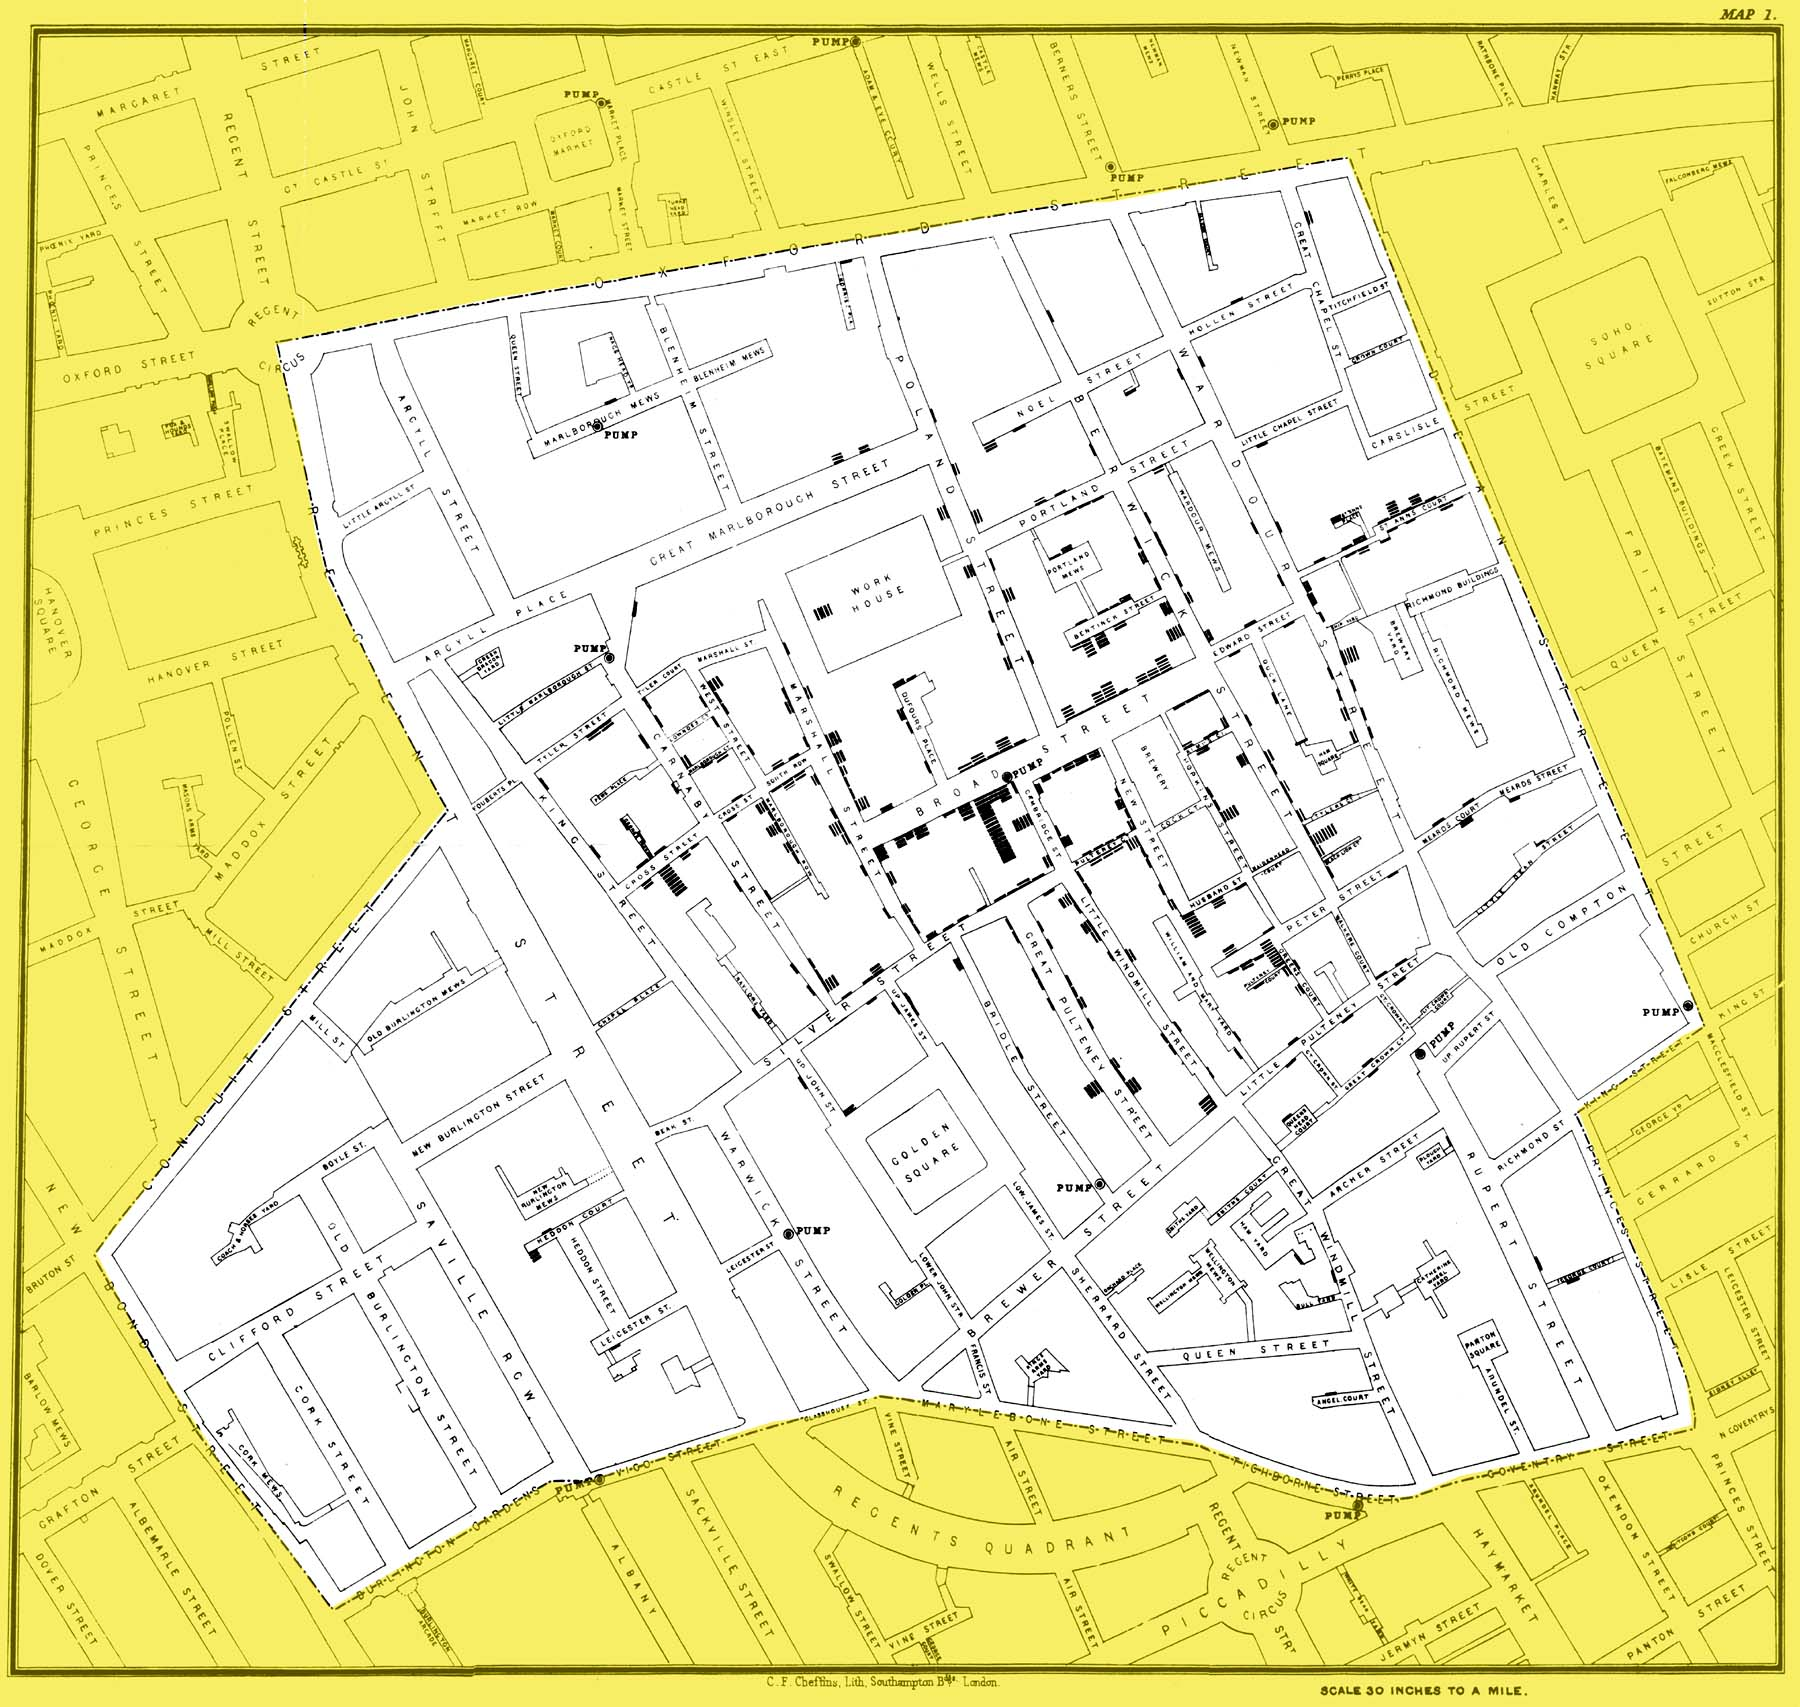
\includegraphics{snowmap_1854}
\caption{Caption}
\label{fig:snow}
\end{figure}

\begin{figure}
\centering
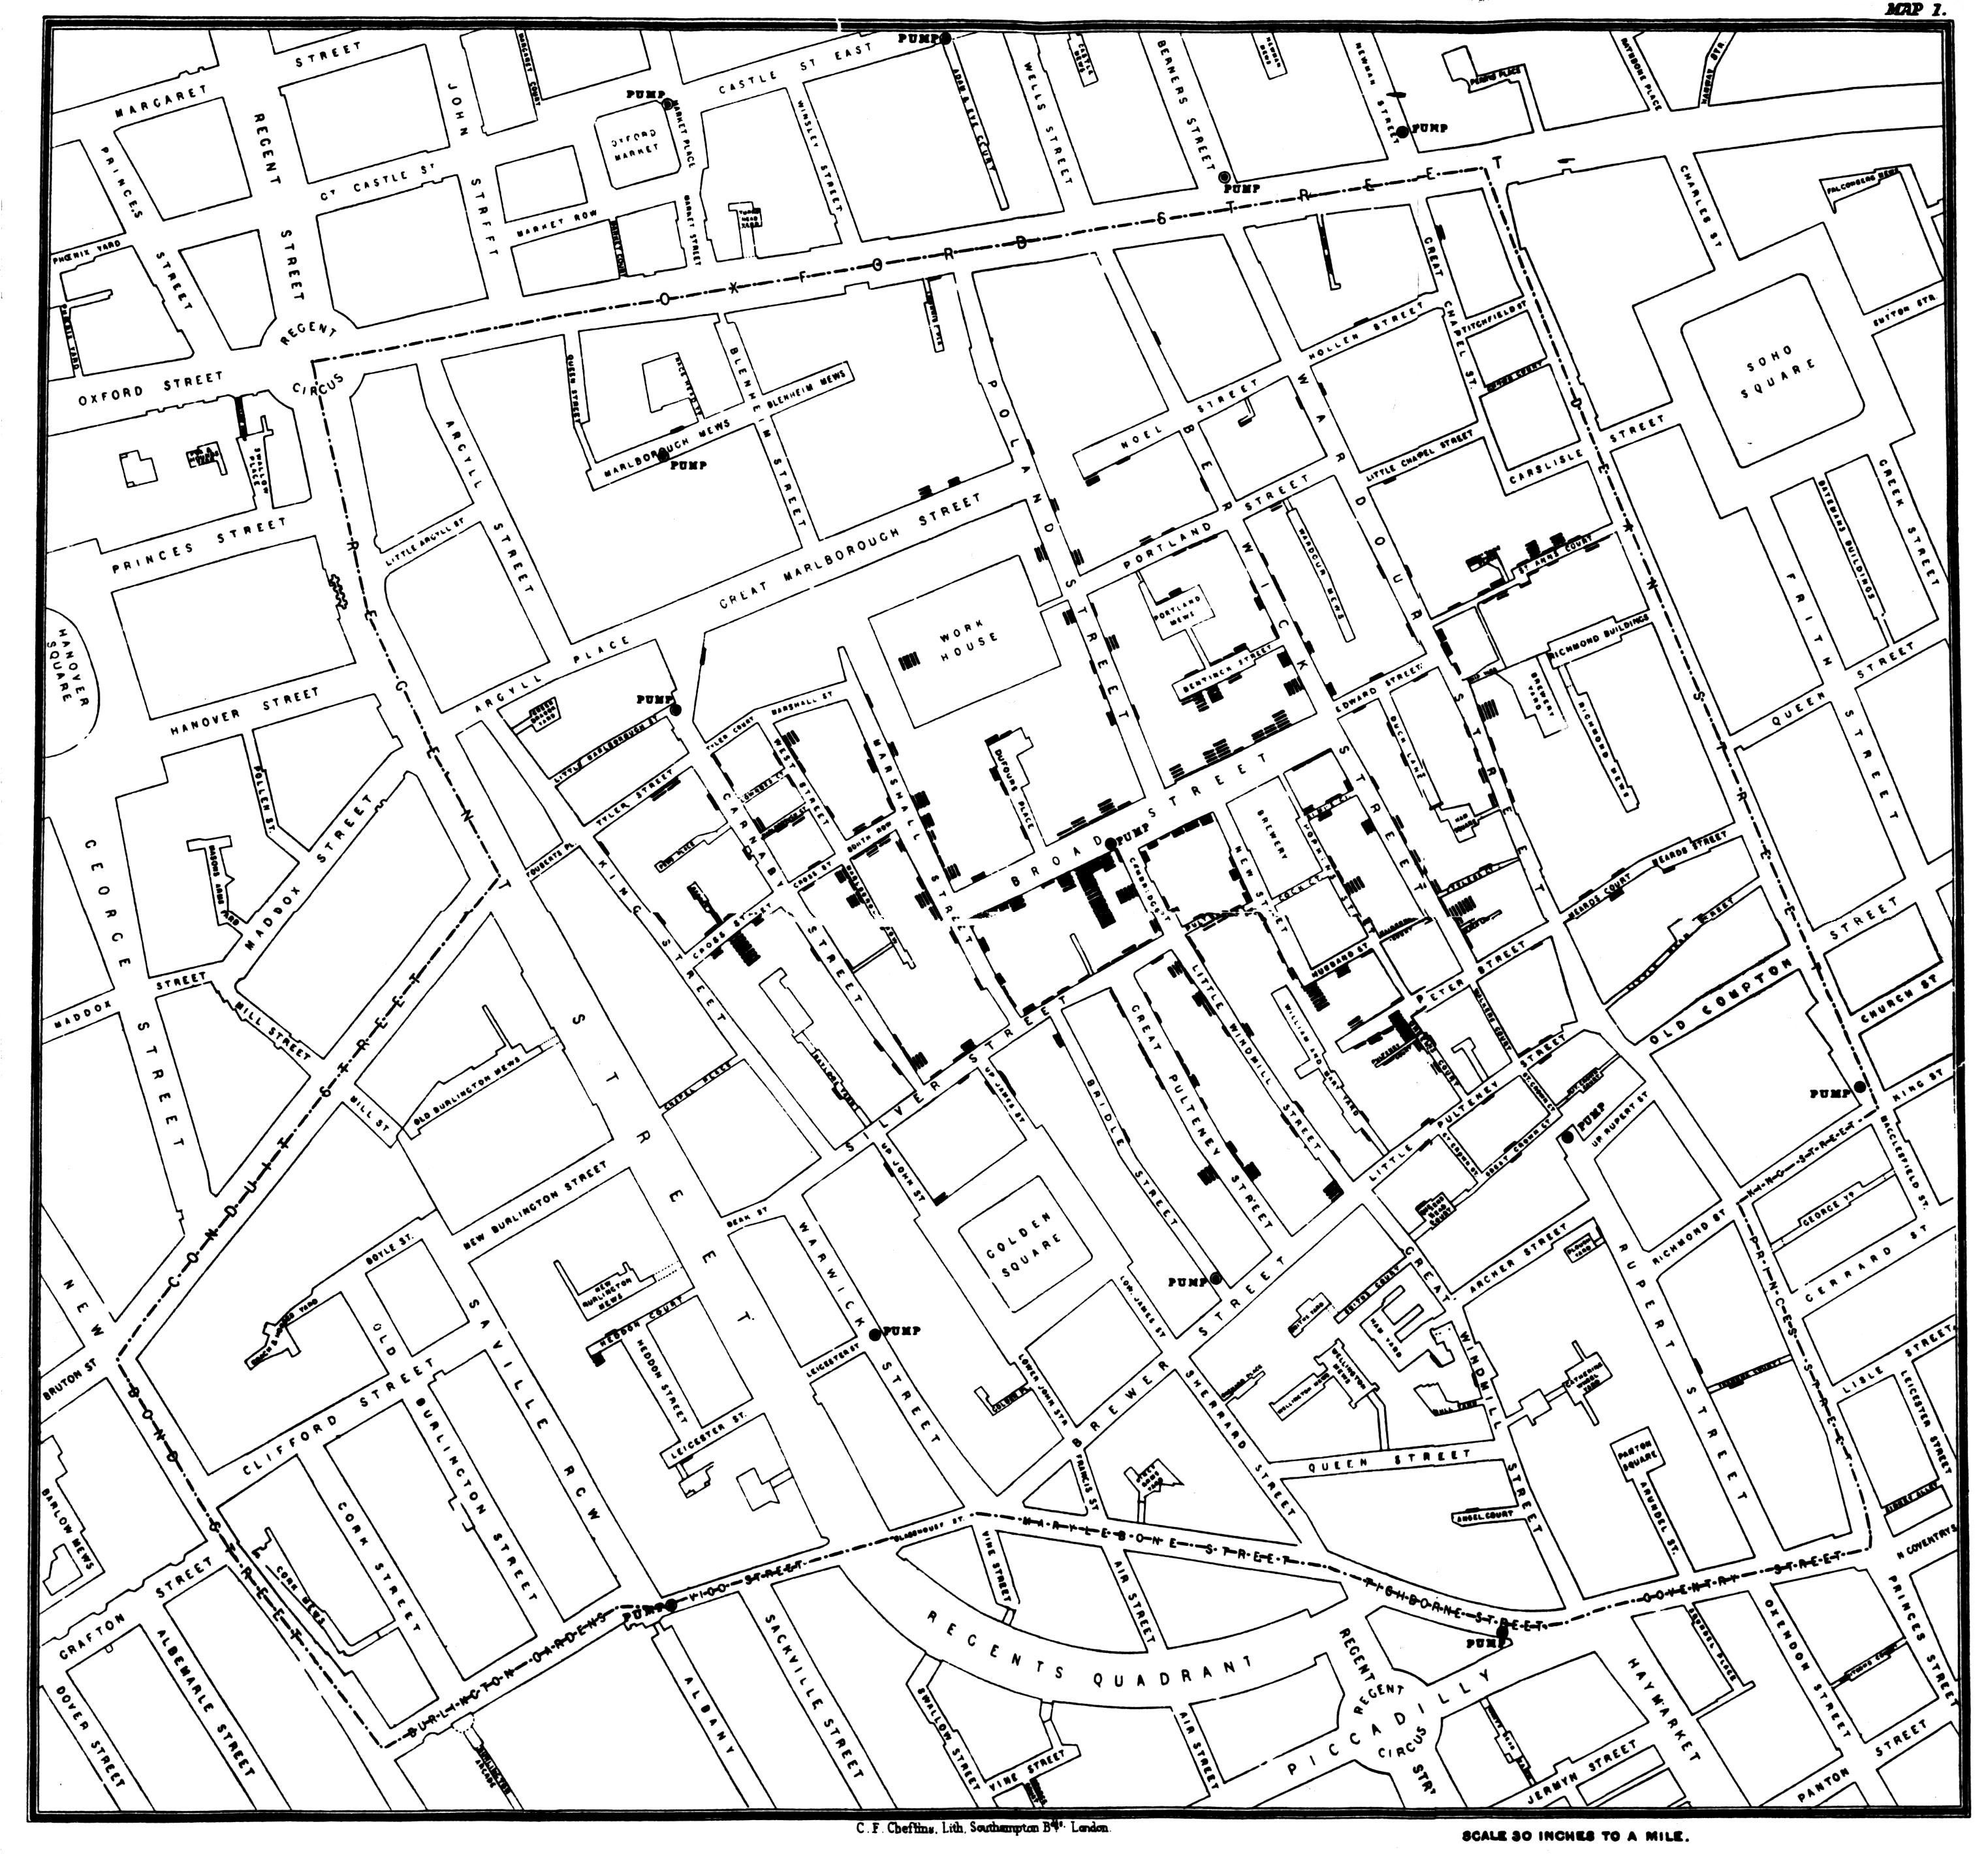
\includegraphics[scale=0.1]{Snow-cholera-map-1}
\caption{John Snow's Cholera map}
\label{fig:snow}
\end{figure}

\section{The Impact/Significance/Influence of Snow's Cholera Map}

John Snow's technique of mapping the spread of disease is still used today. Snow used a scientific approach that contained evidence which was portrayed in an understandable and interpretable way such that anyone could understand it at the time. Snow was able to link evidence from the cholera outbreak, and make logical connections which uncovered meaningful patterns, and told a story \cite{channel1}.Despite all the information being available, no one had used this information to connect the dots, whereas John snow's map enabled a holistic view that explained what was happening \cite{channel1}. 

When he got authorities to remove the handle, it was more symbolic since the Cholera epidemic had pretty much burnt itself anyway. The real significance of John Snow's story was that its the birth of epidemiology, the birth of statistical analysis, and it shows how many lives you can save, improve conditions with proper conditional surveys. \cite{youtube}

His work addressed an ongoing medical debate — in what is widely regarded as one of the most important early examples of epidemiology, he clearly linked cholera’s spread to water instead of air. \cite{blog}

This map that changed the way the world understood cholera. It forced London to realise it needed to build a sewage system to fix itself and end cholera outbreaks. This map makes my top 5 because it was used to convince people of the need for change. \cite{top5}

His map is not only an important historical moment in public health, but also a breakthrough in the visual display of information. By showing abstract medical statistics within a geographic image, a pattern of illness distribution was made visible in a way that pointed to its cause. Today we call such information visualisations Graphic Information Systems (GIS for short). \cite{test}

Steven Johnson, in his book “The Ghost Map” about the London cholera epidemic and efforts to stop it, notes that Snow’s was not the first map to chronicle cholera outbreaks, or even this particular cholera outbreak. \cite{history}

\section{Similar Visualisations in the nineteenth century}
\todo{could be moved to history?}
Among the earliest examples of disease mapping were
two spot maps prepared by Valentine Seaman to illustrate
the distribution of yellow fever in New York
towards the close of the eighteenth century. Shapter2, in
his History of the Cholera in Exeter in 1832 included a dot
map showing the distribution of deaths caused by
cholera. (Figure 1). \cite{howe1970some}

“Part of what made Snow’s map groundbreaking was the fact that it wedded state-of-the-art information design to a scientifically valid theory of cholera’s transmission. It was not the mapmaking technique that mattered; it was the underlying science that the map revealed,” Johnson writes. \cite{history}

It's possible to solve these problems, if we look at the empirical evidence such as the map. ``It's a  map of deaths that ended up creating a whole new way of life, a life that we are enjoying today." \cite{tedtalk}

\todo{from wikipedia}
Snow's study was a major event in the history of public health and geography. It is regarded as the founding event of the science of epidemiology.


\section{Modern Visualisations}
The map could be considered a spot map or a dot map. 

Edward Tufte, a godfather of information display, analyzes this map in his 1997 book, Visual Explanations. Tufte points out that as a dot map, 2 Snow’s visualization is implicitly assuming that the population in the area is uniformly distributed. In other words, a house without any deaths means that the inhabitants of that house successfully avoided cholera, not that the house sits empty. But even with that shortcoming, Tufte praises the map’s usefulness. \cite{blog}

\section{Questions it answers}

John Snow's map evidently answers questions as to how diseases could be visualised. In addition, the statistical scientific approach that Snow had done, contributed to the way in which we view information. Through visualisation, the audience is able to interpret and understand data in a new way. A way, in which is easy to process, compared to standard tables and such. Although John Snow paved the way for epidomology, GIS, and other fields, Snow's map is fairly simple, it may be difficult to apply in a multi-variable context. 


\section{Conclusion}


% \bibliographystyle{IEEEtranN}
% \bibliographystyle{ieeetr}


\bibliography{mybib}
\bibliographystyle{ieeetr}

\end{document}